\documentclass[a4paper, 10pt, conference]{IEEEtran}

\IEEEoverridecommandlockouts

\usepackage[utf8]{inputenc}
\usepackage[T1]{fontenc}
\usepackage[colorlinks=true,linkcolor=black,anchorcolor=black,citecolor=black,filecolor=black,menucolor=black,runcolor=black,urlcolor=black]{hyperref}
\usepackage{graphicx}
\usepackage[ngerman]{babel}
\usepackage[style=ieee]{biblatex}
\usepackage[nolist]{acronym}


\addbibresource{references.bib}

\graphicspath{ {./images/} }

  \begin{acronym}
    \acro{uuid}[UUID]{Universally Unique Identifier}
  \end{acronym}

\begin{document}

\makeatletter
\newcommand{\linebreakand}{%
\end{@IEEEauthorhalign}
\hfill\mbox{}\par
\mbox{}\hfill\begin{@IEEEauthorhalign}
}
\makeatother

\title{\LARGE \bf
Nautical Nonsense: Because Sometimes You Just Need to Sink Something
}

\author{

\IEEEauthorblockN{Jakob Götz} 
\IEEEauthorblockA{\textit{j.goetz@oth-aw.de}}\and
\IEEEauthorblockN{Uwe Kölbel} 
\IEEEauthorblockA{\textit{u.koelbel@oth-aw.de}}\and
\IEEEauthorblockN{Maximilian Schlosser} \IEEEauthorblockA{\textit{m.schlosser@oth-aw.de}}\and
\IEEEauthorblockN{Oliver Schmidts} \IEEEauthorblockA{\textit{o.schmidts@oth-aw.de}}\linebreakand
\IEEEauthorblockN{Jan Schuster} 
\IEEEauthorblockA{\textit{j.schuster@oth-aw.de}}\and
\IEEEauthorblockN{Philipp Seufert} 
\IEEEauthorblockA{\textit{p.seufert@oth-aw.de}}\and
\IEEEauthorblockN{Fabian Wagner} 
\IEEEauthorblockA{\textit{f.wagner@oth-aw.de}}
}

\maketitle
\thispagestyle{empty}
\pagestyle{empty}

\begin{abstract}
Dieser Technical Report beschreibt die Architektur von dem Cloud Native Browser-Game \textit{Nautical Nonsense}.
\end{abstract}


\section{Einleitung}
Schiffeversenken ist seit je her ein beliebtes Spiel. Hauptsächlich wird dieses Spiel jedoch als Brettspiel in Präsenz gespielt. Als 2019 die Corona-Pandemie startete, mussten zwangsweise die Kontakte reduziert werden. Dies ruf eine massive Veränderung in der Lebensweise der Menschen hervor. Besonders im Bereich der Unterhaltung entwickelten sich in kurzer Zeit viele Lösungen, um Aktivitäten, welche zuvor in Präsenz waren, in den Online-Raum zu migrieren. Inspiriert von dieser Entwicklung entstand die Idee, ein Cloud-Nativ Schiffeversenken zu erstellen.\\
In den weiteren Abschnitten dieses Dokuments wird auf die technischen Details des Vorhabens eingegangen. Abschnitt II enthält dabei die Vorgehensweise, welche sicherstellt, dass die Projektziele erreicht werden. Es folgt Abschnitt III, welches einen Überblick über die einzelnen Bausteine gibt und Abschnitt IV, worin die Entwicklungswerkzeuge erläutert werden. Abschließend wird in Abschnitt V auf das Fazit und den Ausblick eingegangen.


\section{Vorgehensweise}\label{sec:vorgehensweise}
Da \textit{Nautical Nonsense} als Cloud-Nativ Browser-Game Anwendung konzipiert ist, ergaben sich bei der Vorgehensweise einige Punkte, welche die Grundlegende Struktur des Projektes und die Umsetzung beeinflusst haben.\\

\textbf{keine Datenpersitenz im Backend} Die Lösungsstrategie im Backend war es eine Kommunikation zu ermöglichen ohne größere Datenmengen darin zu speichern. Da \textit{Nautical Nonsense} als Cloud-Native Anwendung konzipiert wurde, durfte die persitenz der Daten nicht im Backend gehalten werden. Dies wurde gelöst, indem die Verarbeitung der Daten im Backend erfolgt, jedoch direkt im Anschluss eine Speicherung in der Datenbank vorgenommen wird. 

\textbf{Herausforderungen im Frontend} 
ein Text welcher die Vorgehensweise, Herausforderungen und Lösungswege beschreibt\\
\textbf{Herausforderungen in der Datenbank} 
ein Text welcher die Vorgehensweise, Herausforderungen und Lösungswege beschreibt\\
\textbf{Herausforderungen in der Infrastruktur} 
ein Text welcher die Vorgehensweise, Herausforderungen und Lösungswege beschreibt\\

\section{Bausteinsicht}\label{sec:bausteinsicht}



\subsection{Datenbank}\label{subsec:datenbank}
Zur dauerhaften Speicherung aller Daten, die während des Spiels anfallen, wird die NoSQL-Datenbank \textit{MongoDB} verwendet. Um den Implementierungsaufwand zu reduzieren, wird dabei auf das Cloudangebot \textit{MongoDB Atlas} zurückgegriffen. In der Datenbank werden JSON-artige Dokumente in einzelnen Collections abgelegt, die für je eine bestimmte Funktion zuständig sind. Tabelle~\ref{tab:collections} zeigt eine Übersicht über die vorhandenen Collections.

\begin{table}[h!]
    \begin{center}
        \caption{Collections}
        \label{tab:collections}
        \begin{tabular}{|l|l|}
            \textbf{collection} & \textbf{Beschreibung}\\
            \hline
            \texttt{games}				& Aktuelle Spielzustände\\
            \texttt{leaderboard}					& Bestenliste\\
            \texttt{stats}	& Spielstatistiken\\
        \end{tabular}
    \end{center}
\end{table}

In \texttt{games} werden die aktuellen Spielstände jedes Spiels gespeichert. Hierzu gehören neben einer eindeutigen Game-ID Informationen zu den Spielern, deren momentane Spielfelder sowie getroffene und versenkte Schiffe.

Ist ein Spiel zu Ende, wird der Gewinner zusammen mit seiner benötigten Zuganzahl in \texttt{leaderboard} gespeichert. Außerdem werden Daten zu Kapitulation und Gegner (Mensch oder Computer) ergänzt, sodass im Frontend zwei getrennte Bestenlisten angezeigt werden können.

Die Spielstatistiken werden ebenso nach jedem beendeten Spiel aktualisiert. Ein Dokument in \texttt{stats} enthält dabei Daten zu bereits abgeschlossenen Spielen, wie Spielanzahl und durchschnittliche Schusszahl - getrennt nach Mensch- und Computergegner. Zusätzlich werden häufige Schiffs- und Schusspositionen sowie die Abschussquote der einzelnen Schiffstypen protokolliert.

\subsection{Backend}\label{subsec:backend}
Das Backend ist mit Python und den Framework FastAPI~\cite{fastapi} umgesetzt. Das Frontend kommuniziert mit dem Backend über zwei Schnittstellen. Zum einen über die RESTful-API, zum anderen über eine Websocket Verbindung. Die RESTful-API übernimmt alle Anfragen des Frontends, welche nicht die Kommunikation zwischen zwei Spieler betrifft. Somit dient die RESTful-API hauptsächlich als Knotenpunkt zur Datenbank. Die Websocket Schnittstelle dient zur Kommunikation zwischen zwei Frontends. Die Kommunikationsdaten der Websocket-Verbindung werden im Backend aufbereitet, validiert und in der Datenbank gespeichert. Darauf folgt eine sofortige Antwort an beide Frontends, um diese über den neuen Spielschritt zu informieren.

Folgende HTTP-Endpunkte, in Tabelle~\ref{tab:api}, stellt die API im Backend für das Frontend zur Verfügung:

\begin{table}[h!]
    \begin{center}
        \caption{RESTful-API}
        \label{tab:api}
        \begin{tabular}{|l|l|}
            \textbf{Endpunkt} & \textbf{Beschreibung}\\
            \hline
            \texttt{GET \, /}				& Startseite\\
            \texttt{POST /play}					& Starten eines neuen Spiels\\
            \texttt{WEBSOCKET /ws/}\detokenize{{client_id}}	& Kommunikation der Spieler\\
            \texttt{GET /leaderboard}	& Daten für das Leaderboard\\
	    \texttt{GET /stats}	& Daten für Spielstatistiken\\
        \end{tabular}
    \end{center}
\end{table}


Die \texttt{/}-Route gibt eine \ac{uuid} als String zurück, welche das Frontend nutzen kann, um den Spieler gegenüber des Backends bei nachfolgenden Anfragen eindeutig zu bestimmen. Ein Spiel wird mit der \texttt{/play}-Route gestartet. Diese Route nimmt ein JSON-Objekt entgegen, in welchen spezifiziert wird, welchen Spielmodus der Spieler spielen möchte. Als Rückgabe bekommt das jeweilige Frontend eine Ready-Flag und die \ac{uuid} der beiden Kontrahenten. Nachdem ein Spiel bereit ist, wird die Websocket Verbindung über die \texttt{/ws/}-Route aufgebaut. Über diese Route läuft die komplette Kommunikation bis zum Spielende.

\begin{figure}[thp]
    \centering
    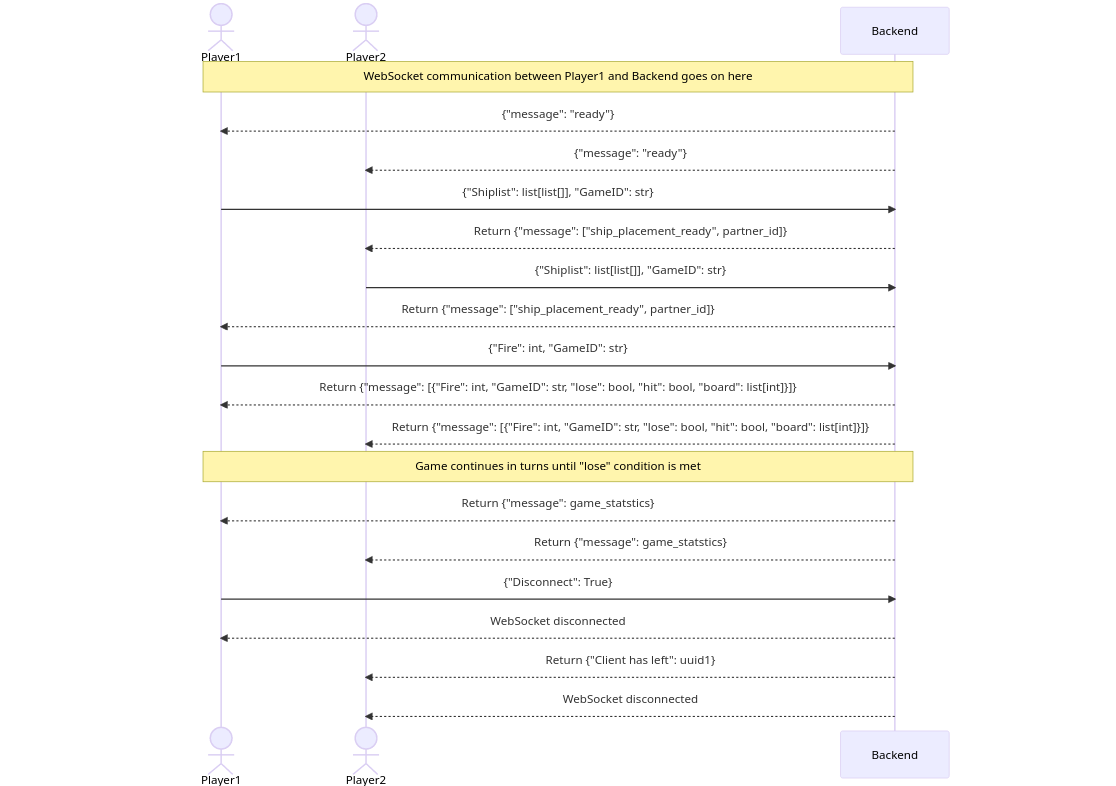
\includegraphics[width=\linewidth]{websocket_comm}
    \caption{Websocket Kommunikation}
    \label{fig:websocket_comm}
\end{figure}

\subsection{Frontend}\label{subsec:frontend}

\subsubsection{Kommunikation mit Backend}\label{subsec:comwithbackend}

Beim Aufrufen der Webseite sendet der Client einen HTTP-GET-Request an \glqq localhost:8000\grqq{} und erhält ein JSON-Objekt mit der Client-ID. Diese ID wird der globalen Variable \textit{sharedData.clientID} zugewiesen.

Die Websocket-Verbindungs-URL wird durch das Hinzufügen der Client-ID zu \textit{sharedData.websocket\_url} erstellt.

Wenn der Client in der Start-Szene \glqq Spiel gegen Random\grqq{} auswählt, erfolgt ein HTTP-POST-Request an \glqq localhost:8000/play\grqq{} mit Informationen wie der Client-ID, dem ausgewählten Modus und dem Spielernamen. Die empfangene Game-ID wird in \textit{sharedData.game\_id} gespeichert.

Die Websocket-Verbindung wird erst nach erfolgreicher Ausführung dieses Befehls initialisiert, bevor zur Szene \glqq Waiting1\grqq{} gewechselt wird. Dieser Websocket existiert ebenfalls als globale Variable namens \textit{sharedData.socket}.

In allen Szenen ist die Methode \textit{onmessage} implementiert, die es ermöglicht, über Websockets eingehende Nachrichten vom Backend zu empfangen. Diese Methode ist Bestandteil des JavaScript-Objekts \textit{WebSocket}.

Wenn sich ein zweiter Client auf der Webseite verbindet und die Option \glqq Spiele gegen Random\grqq{} auswählt, sendet das Backend über die Websocket-Verbindung ein \glqq ready\grqq{}-Flag an beide Clients. In Folge dessen wird die Variable \textit{sharedData.ready} auf den Wert \glqq true\grqq{} gesetzt und es erfolgt ein nahtloser Wechsel zur Szene \glqq Shipplacement\grqq{}.

In dieser Szene wird die Platzierung der Schiffe (Positionen) und die Game-ID an das Backend über die Websocket-Verbindung übermittelt. Für das Senden wird zuerst überprüft, ob die Websocket-Verbindung steht und anschließend die Methode \textit{JSON.stringify} verwendet, um ein JSON-Objekt in einen JSON-String zu konvertieren. Dieser wird anschließend mittels \textit{sharedData.socket.send(JSON-String)} an das Backend gesendet.

 Die grundlegende Vorgehensweise beim Empfangen und Senden von Nachrichten via Websockets ändert sich in den restlichen Szenen nicht. Es wurde lediglich die Verarbeitung der Daten auf den jeweiligen Use-Case angepasst. In Abbildung \ref{fig:websocket_comm} ist ein Schaubild der Websocket Kommunikation ersichtlich.





\subsection{Infrastruktur}\label{subsec:infrastruktur}





\section{Entwicklungswerkzeuge}\label{sec:entwicklungswerkzeuge}



\subsection{Backend}\label{subsec:backend-dev-tools}
Das Backend wird hauptsächlich mit FastAPI implementiert, einem Framework, das auf "Starlette"~\cite{starlette} und "Pydantic"~\cite{pydantic} aufbaut. Starlette stellt Funktionen wie WebSockets zur Verfügung, während Pydantic die Validierung von Datenmodellen ermöglicht, die von FastAPI verwendet werden. Dank Starlette kann auch das Test-Framework "Pytest"~\cite{pytest} direkt für Unit-Tests eingesetzt werden. Der Asynchronous Server Gateway Interface (ASGI) Server "Uvicorn"~\cite{unvicorn} wird für die Bereitstellung genutzt.
%TODO @Fabi willst da vllt noch was dazu schreiben?
Für den Zugriff auf die Mongo-Datenbank wird das Framework PyMongo genutzt. 




\subsection{Frontend}\label{subsec:frontend-dev-tools}



\section{Fazit und Ausblick}\label{sec:fazit}




\printbibliography

\end{document}

